% !TEX root = ../master-thesis.tex

\textbf{Role of imaging in fast-cycle experiments.}  
In high-repetition quantum simulation experiments with ${}^6$Li, fast, minimally disruptive, and high-fidelity single-atom detection is essential. Free-space imaging~\cite{bergschneider_spin-resolved_2018,su_fast_2025} offers a simple and efficient alternative to traditional Raman-based fluorescence imaging. In this method, atoms are released from their traps and illuminated with resonant light. Fluorescence is collected without requiring additional cooling or deep pinning potentials. The short exposure time, typically around $10~\mu$s, allows for much higher experimental repetition rates compared to standard approaches based on quantum gas microscopes.

\textbf{Free-space imaging for ${}^6$Li.}  
Although ${}^6$Li is a light atom and experiences relatively large momentum recoil during scattering, its broad D2 transition at $\lambda = 671$~nm allows for rapid photon emission. The typical recoil velocity is given by $v_\mathrm{rec} = {h}/{m \lambda}$, where $m$ is the atomic mass of ${}^6$Li and $\lambda$ is the wavelength of the imaging light. As the atom scatters photons at a rate $\Gamma$, each with random emission direction, it undergoes a random walk in momentum space. This results in spatial diffusion during the imaging pulse. The root-mean-square width of this random walk is approximately \cite{kruip_design_2024} (in the flashing regime)
\begin{equation}
	\sigma_\mathrm{rw} = \tfrac{1}{3} v_\mathrm{rec} \Gamma^{1/2} t^{3/2},
	\label{eq:sigmarw}
\end{equation}
where $t$ is the total exposure time. For a fixed number of scattered photons $N_\mathrm{ph}$, we can express $t = N_\mathrm{ph} / \Gamma$, yielding
\begin{equation}
	\sigma_\mathrm{rw} = \tfrac{1}{3} v_\mathrm{rec} \Gamma^{-1} N_\mathrm{ph}^{3/2}.
\end{equation}

This scaling highlights the trade-off between collecting more fluorescence photons and maintaining spatial resolution. In our system, with $N_\mathrm{ph} \sim 300$, the resulting diffusion is on the scale of $10~\mu$m.
% making single-atom detection feasible 


\begin{figure}[htb]
    \centering
    \addletter{140}{a}
    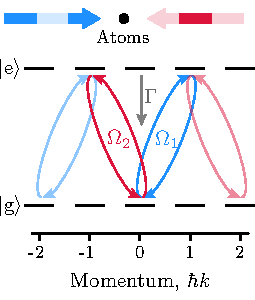
\includegraphics{fig-ai/ssh-scheme.pdf}
    \hfill
    \addletter{140}{b}
    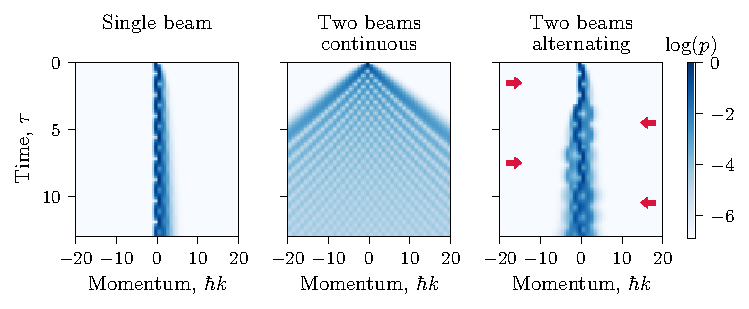
\includegraphics{fig-py/ssh-model.pdf}
    \caption{
        \textbf{Momentum-space dynamics in the SSH model}. 
        a) Atoms undergo momentum-changing transitions via couplings $\Omega_1$ and $\Omega_2$, realizing a SSH-like quantum walk.
        b) Momentum distributions over time for different beam configurations: single beam (left) shows small shift; two continuous beams (middle) result in fast spreading; alternating beams (right) suppress spread.
    }
    \label{fig:sshmodel}
\end{figure}


\textbf{Connection to the SSH model.}  
The scattering dynamics of a freely moving atom illuminated by resonant counter-propagating beams can be understood as a momentum-space quantum walk. This process maps onto the Su-Schrieffer-Heeger (SSH) model:
\begin{equation*}
	H = t_1 \sum_n \ket{n,B}\bra{n,A} + t_2 \sum_n \ket{n+1,A}\bra{n,B} + \text{h.c.}
\end{equation*}
In the atomic case, the model takes the form:
\begin{equation*}
	H = \frac{\Omega_1}{2} \sum_p \ket{p,g}\bra{p+1,e} + \frac{\Omega_2}{2} \sum_p \ket{p-1,e}\bra{p,g} + \text{h.c.}
\end{equation*}
Here, $\Omega_1$ and $\Omega_2$ correspond to the Rabi frequencies of the two beams. When both beams are on simultaneously, the atom undergoes coherent transitions between distant momentum states. This leads to rapid delocalization in space. The evolution can be simulated by solving a Lindblad master equation,
\begin{equation*}
	i \hbar \partial_t \rho = [H(t), \rho] + \mathcal{L}[\rho],
\end{equation*}
with $\mathcal{L}$ describing spontaneous emission. These simulations show that applying the two beams alternately—rather than simultaneously—dramatically suppresses spatial diffusion and improves imaging fidelity (Fig.~\ref{fig:sshmodel}).

\textbf{Spin-resolved imaging with stretched states.}  
To perform spin-resolved detection with high signal strength, atoms are transferred into stretched states $\ket{3}$ and $\ket{6}$ before imaging. These states are nearly pure $m_J = \pm 1/2, m_I = \mp 1$ at high magnetic fields and couple strongly to $\sigma^\pm$ polarized light. Unlike the commonly used $\ket{1}$ and $\ket{2}$ states, which have small admixtures that allow decay into dark states, $\ket{3}$ and $\ket{6}$ support nearly closed cycling transitions. As a result, atoms in these states scatter significantly more photons, often nearly twice as many, which greatly improves detection efficiency.

To distinguish the two spin states during a single imaging pulse, their respective fluorescence is spatially separated on the camera. This is achieved by using a polarizing beam splitter (PBS) after the objective, which directs $\sigma^+$ and $\sigma^-$ components to different regions of the detector (see Fig.~\ref{fig:spin-resolved}). By analyzing the relative photon counts in these regions, one can assign the spin state of each detected atom with high fidelity, as described in Sec.~\ref{subsec:imaging-spin}.

\textbf{Overview of this section.}  
The following subsections describe the complete implementation of spin-resolved free-space imaging in our experiment. Section~\ref{subsec:imaging-setup} details the optical setup built and aligned during this work. Section~\ref{subsec:imaging-processing} explains the image analysis pipeline, which was developed as part of this thesis. Finally, Section~\ref{subsec:imaging-spin} presents the spin-state discrimination method and evaluates its fidelity using experimental calibration data. Together, these elements form a robust and fast readout protocol for our ${}^6$Li tweezer-based simulator.



% Мы работаем с Li6, делаем fast cycle quantum simulator, так что free space imaging предложенный в \cite{bergschneider_spin-resolved_2018} является для нас отличным кандидатом: быстро, просто в реализации (за исключением MWM), spin-resolved. Да, из-за размытия, сам по себе имеет разрешающую способность около 10$\mu$m для Li6 (в контексте нашего эксперимента), так что lattice single-site resolved imaging требует дополнительно использования Matter Wave Magnifier, но мы и будем его использовать а численное моделирование можно найти дальше у меня в дипломе. Но для нас на данном этапе этот метод отлично работал для фотографирования атомов в tweezers, так как можем сами расположить на достаточно для single site imaging. 


% Тут пригодятся эти картинки:


% \begin{figure}[h]
%     \centering
%     \addletter{200}{a}
%     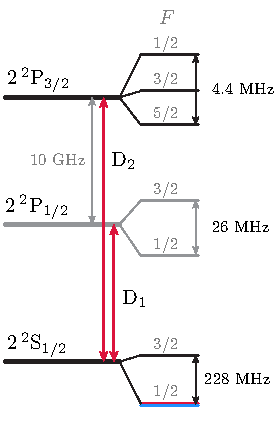
\includegraphics{fig-ai/li-levels-base.pdf}
%     \hspace{1cm}
%     \addletter{200}{b}
%     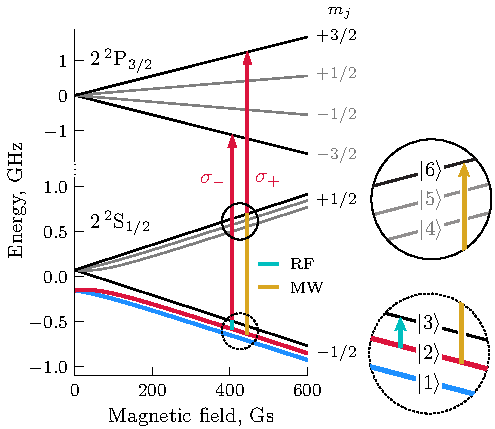
\includegraphics{fig-ai/li6-zeeman-broken-ai.pdf}
%     \caption{
%         \textbf{${}^6$Li energy levels}. 
%         a) Level diagram of the ground and excited states of ${}^6$Li \cite{gehm_preparation_2003}, including the D1 and D2 transitions around $\lambda = 671$~nm. 
%         b) Zeeman splitting of the hyperfine levels of the $2\, {}^2\mathrm{S}_{1/2}$ and $2\, {}^2\mathrm{P}_{2/2}$ in ${}^6$Li \cite{serwane_deterministic_2011, sibalic_arc_2017}. As different spin states for physics we consider state $\ket{1}$ and $\ket{2}$, but for imaging it is worth to flip them to stretched states $\ket{6}$, $\ket{3}$. Colored lines indicate transitions driven by radiofrequency (RF) and microwave (MW) fields.
%     }
%     \label{fig:li6levels}
% \end{figure}


% \begin{figure}[h]
%     \centering
%     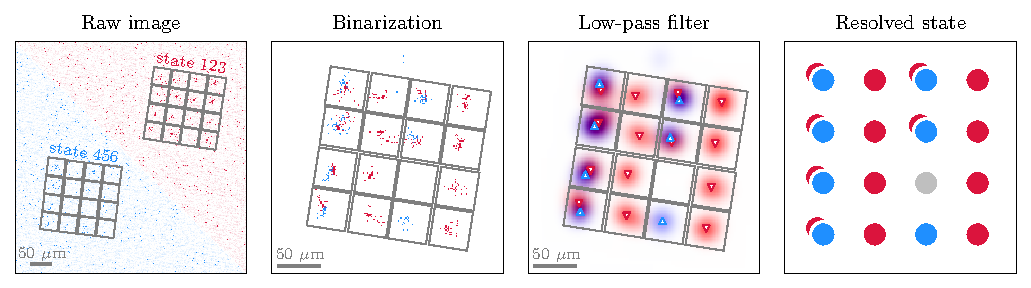
\includegraphics{fig-py/imaging-spin-resolved.pdf}
%     \caption{
%         \textbf{Spin-resolved single-atom imaging.}
%         Spatially separated $\sigma_+$ and $\sigma_-$ fluorescence is imaged onto two distinct regions of the camera. The binarization step identifies photon counts above a threshold, followed by a low-pass filter to extract spatially localized signals. Final spin states are assigned based on relative signal strength in each channel:
%         \raisebox{-1pt}{\scalebox{1.5}{\textcolor{ublue}{\textbullet}}} -- $\ket{1}$, 
%         \raisebox{-1pt}{\scalebox{1.5}{\textcolor{ured}{\textbullet}}} -- $\ket{2}$, 
%         \raisebox{-1pt}{\scalebox{1.5}{\textcolor{uhole}{\textbullet}}} -- no atom.
%     }
%     \label{fig:spin-resolved}
% \end{figure}


% В чем заключался мой вклад? Я реализовал оптическую схему, которая работает на 17 mW мощности одного лазера 671 нм (aka imaging), и выдаёт в каждый из flashing лучей 1 mW мощности (соответствуя в итоге $\sub{s}{sat} \sim 5$). И \red{X} mW другого лазера 671 нм (aka RFA). На схеме примерно 1 mW "imaging laser" идёт на стабилизацию, остальное проходит через контролирующие AOM (для вкл выкл, это Gooch & Housego 3080-120 на 80 MHz x2), beam spliiter (там же лучи RFA и Imaging совмещаются) и разделяются на left and right optical beams (imaging надо делать с двух сторон) и проходят через "flashing" aom (Gooch & Housego 3110-120 на 80 MHz x2), упровляемые через генератор сигналов (Rigol) на который и подаём ступеньки с периодом 1MHz, и потом уже заводятся в оптоволокно. Для повышения эффективности enabling AOM перед ними стоит линза 1000mm (LA1464-B). Два лазера используются, так как для spin resolve imaging нам нужно  работать с двумя переходами, отстоящими на 0.5 GHz. 




% \begin{figure}[h]
%     \centering
%     \addletter{195}{a} \phantom{4}
%     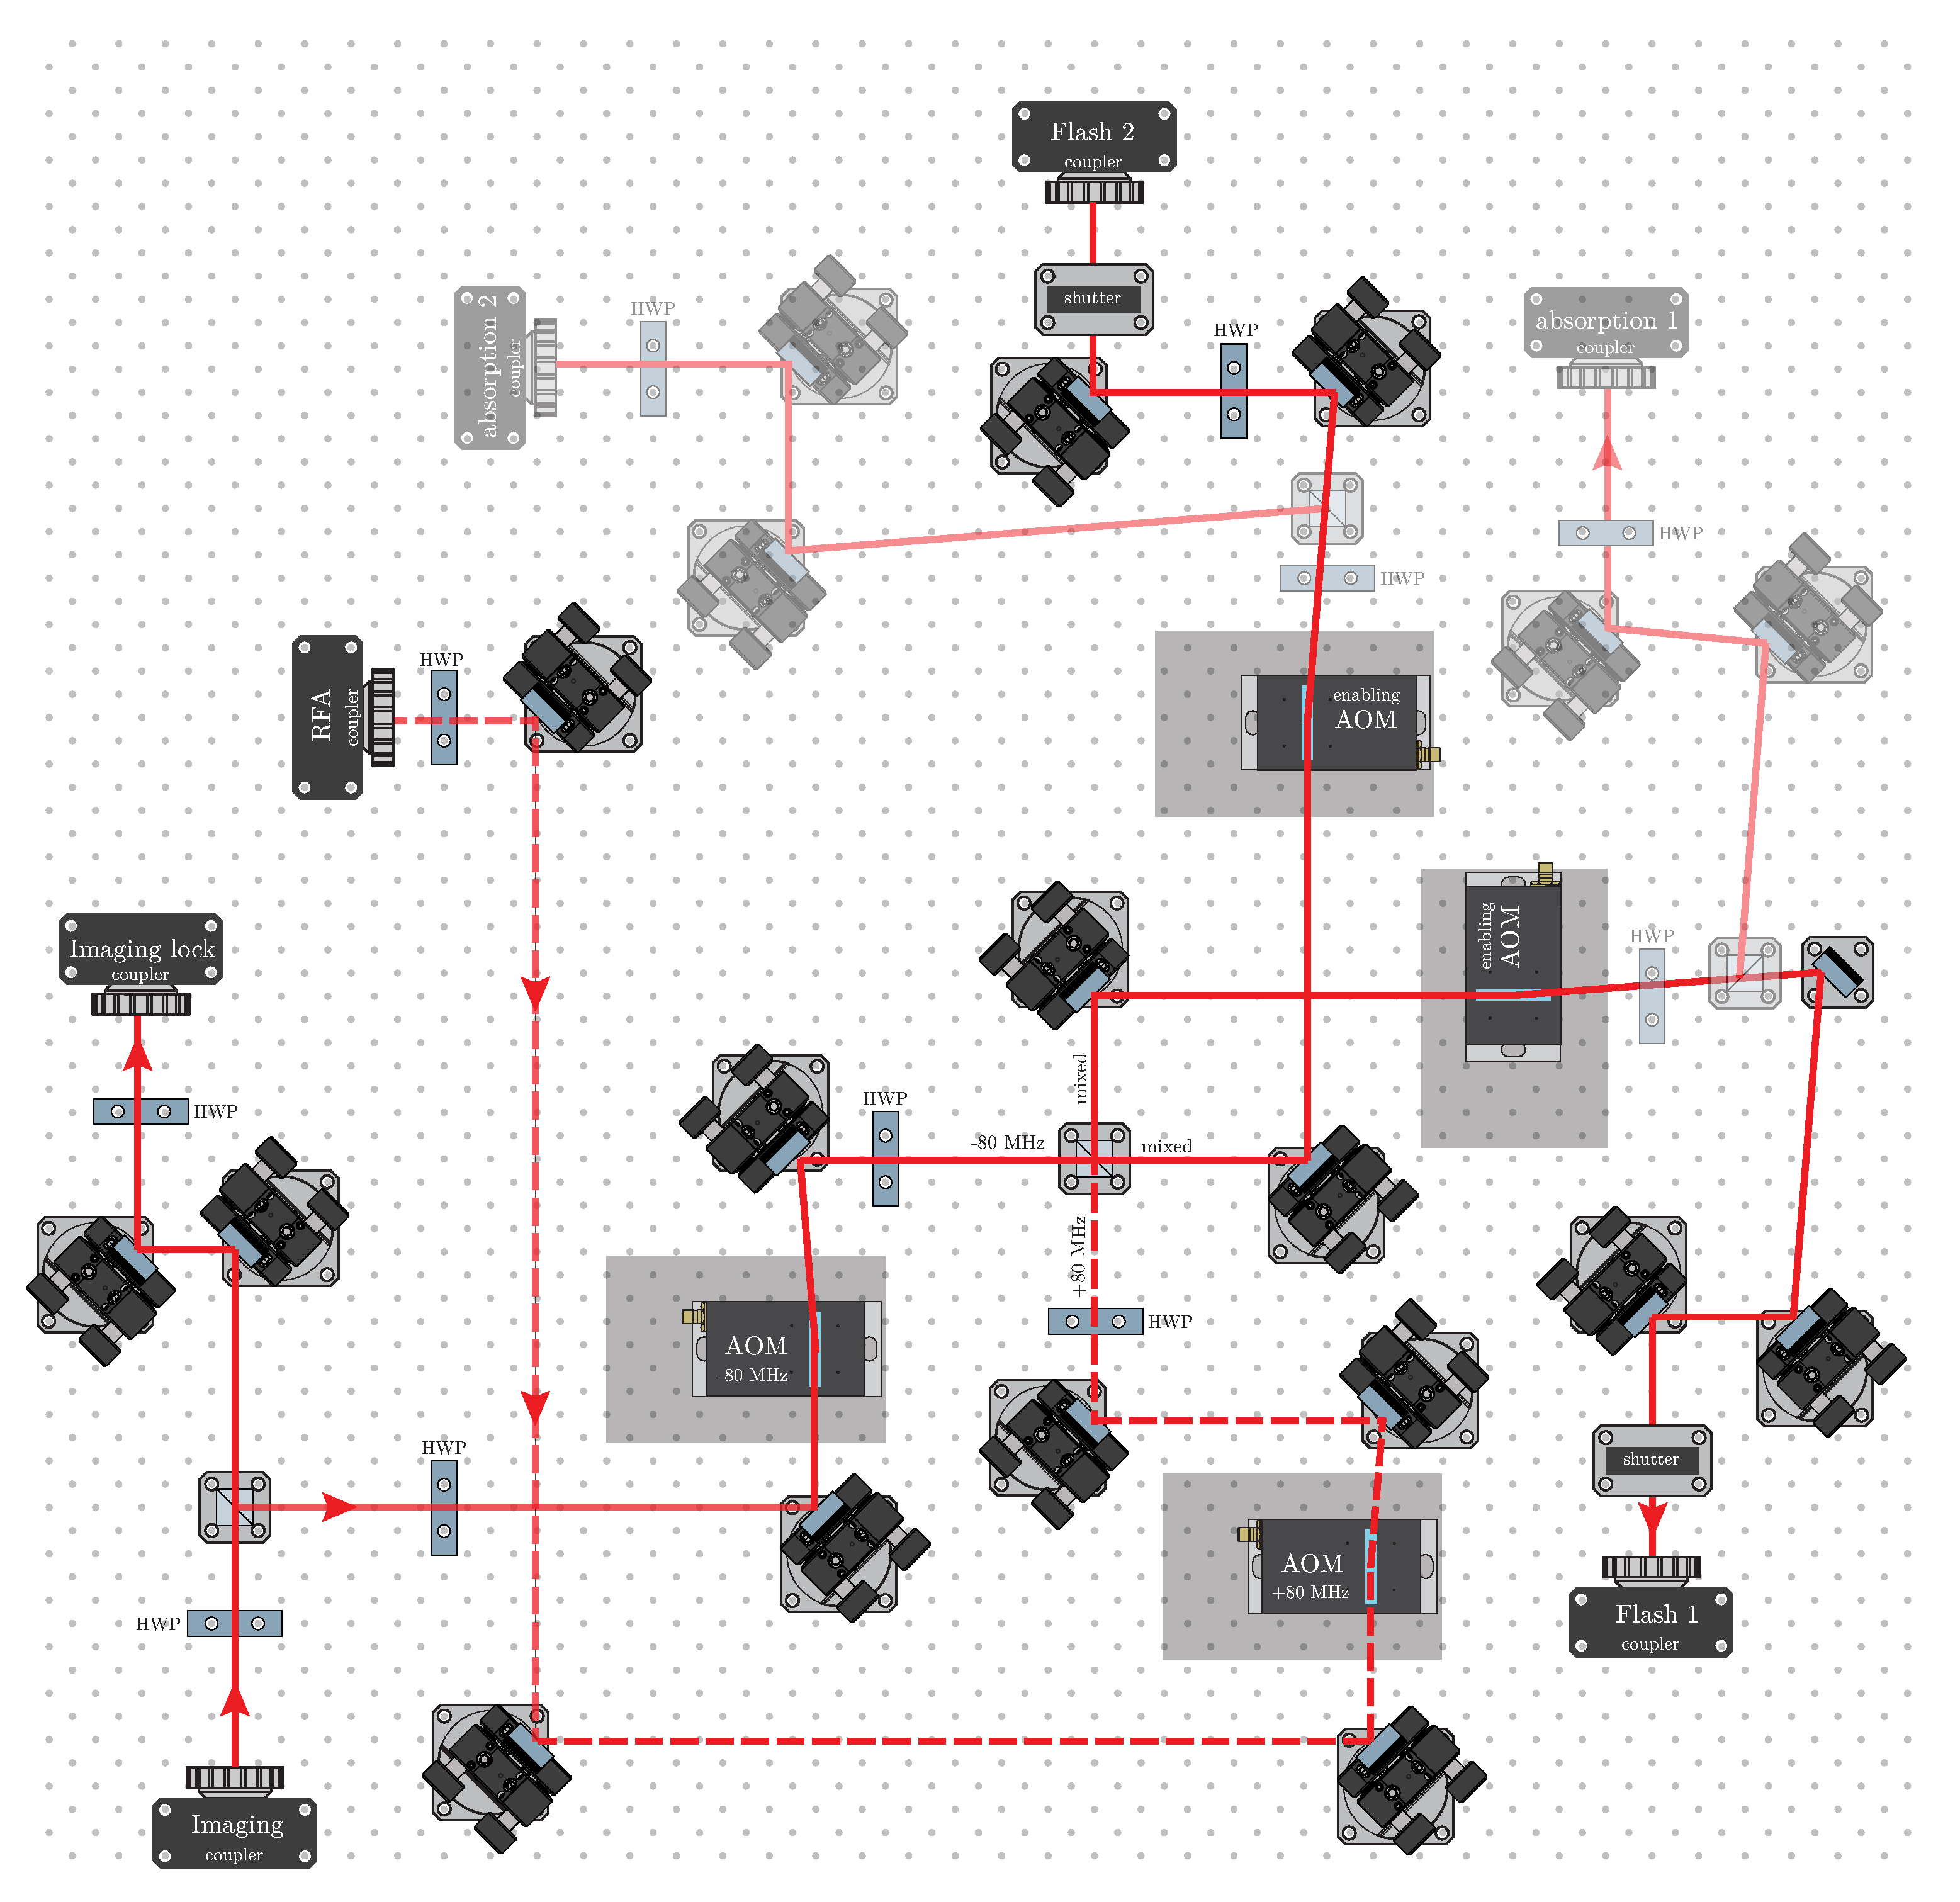
\includegraphics[width=0.4\textwidth]{fig-ai/flashing-distribution-scheme.pdf}
%     \hspace{10 mm} 
%     \addletter{195}{b} \phantom{4}
%     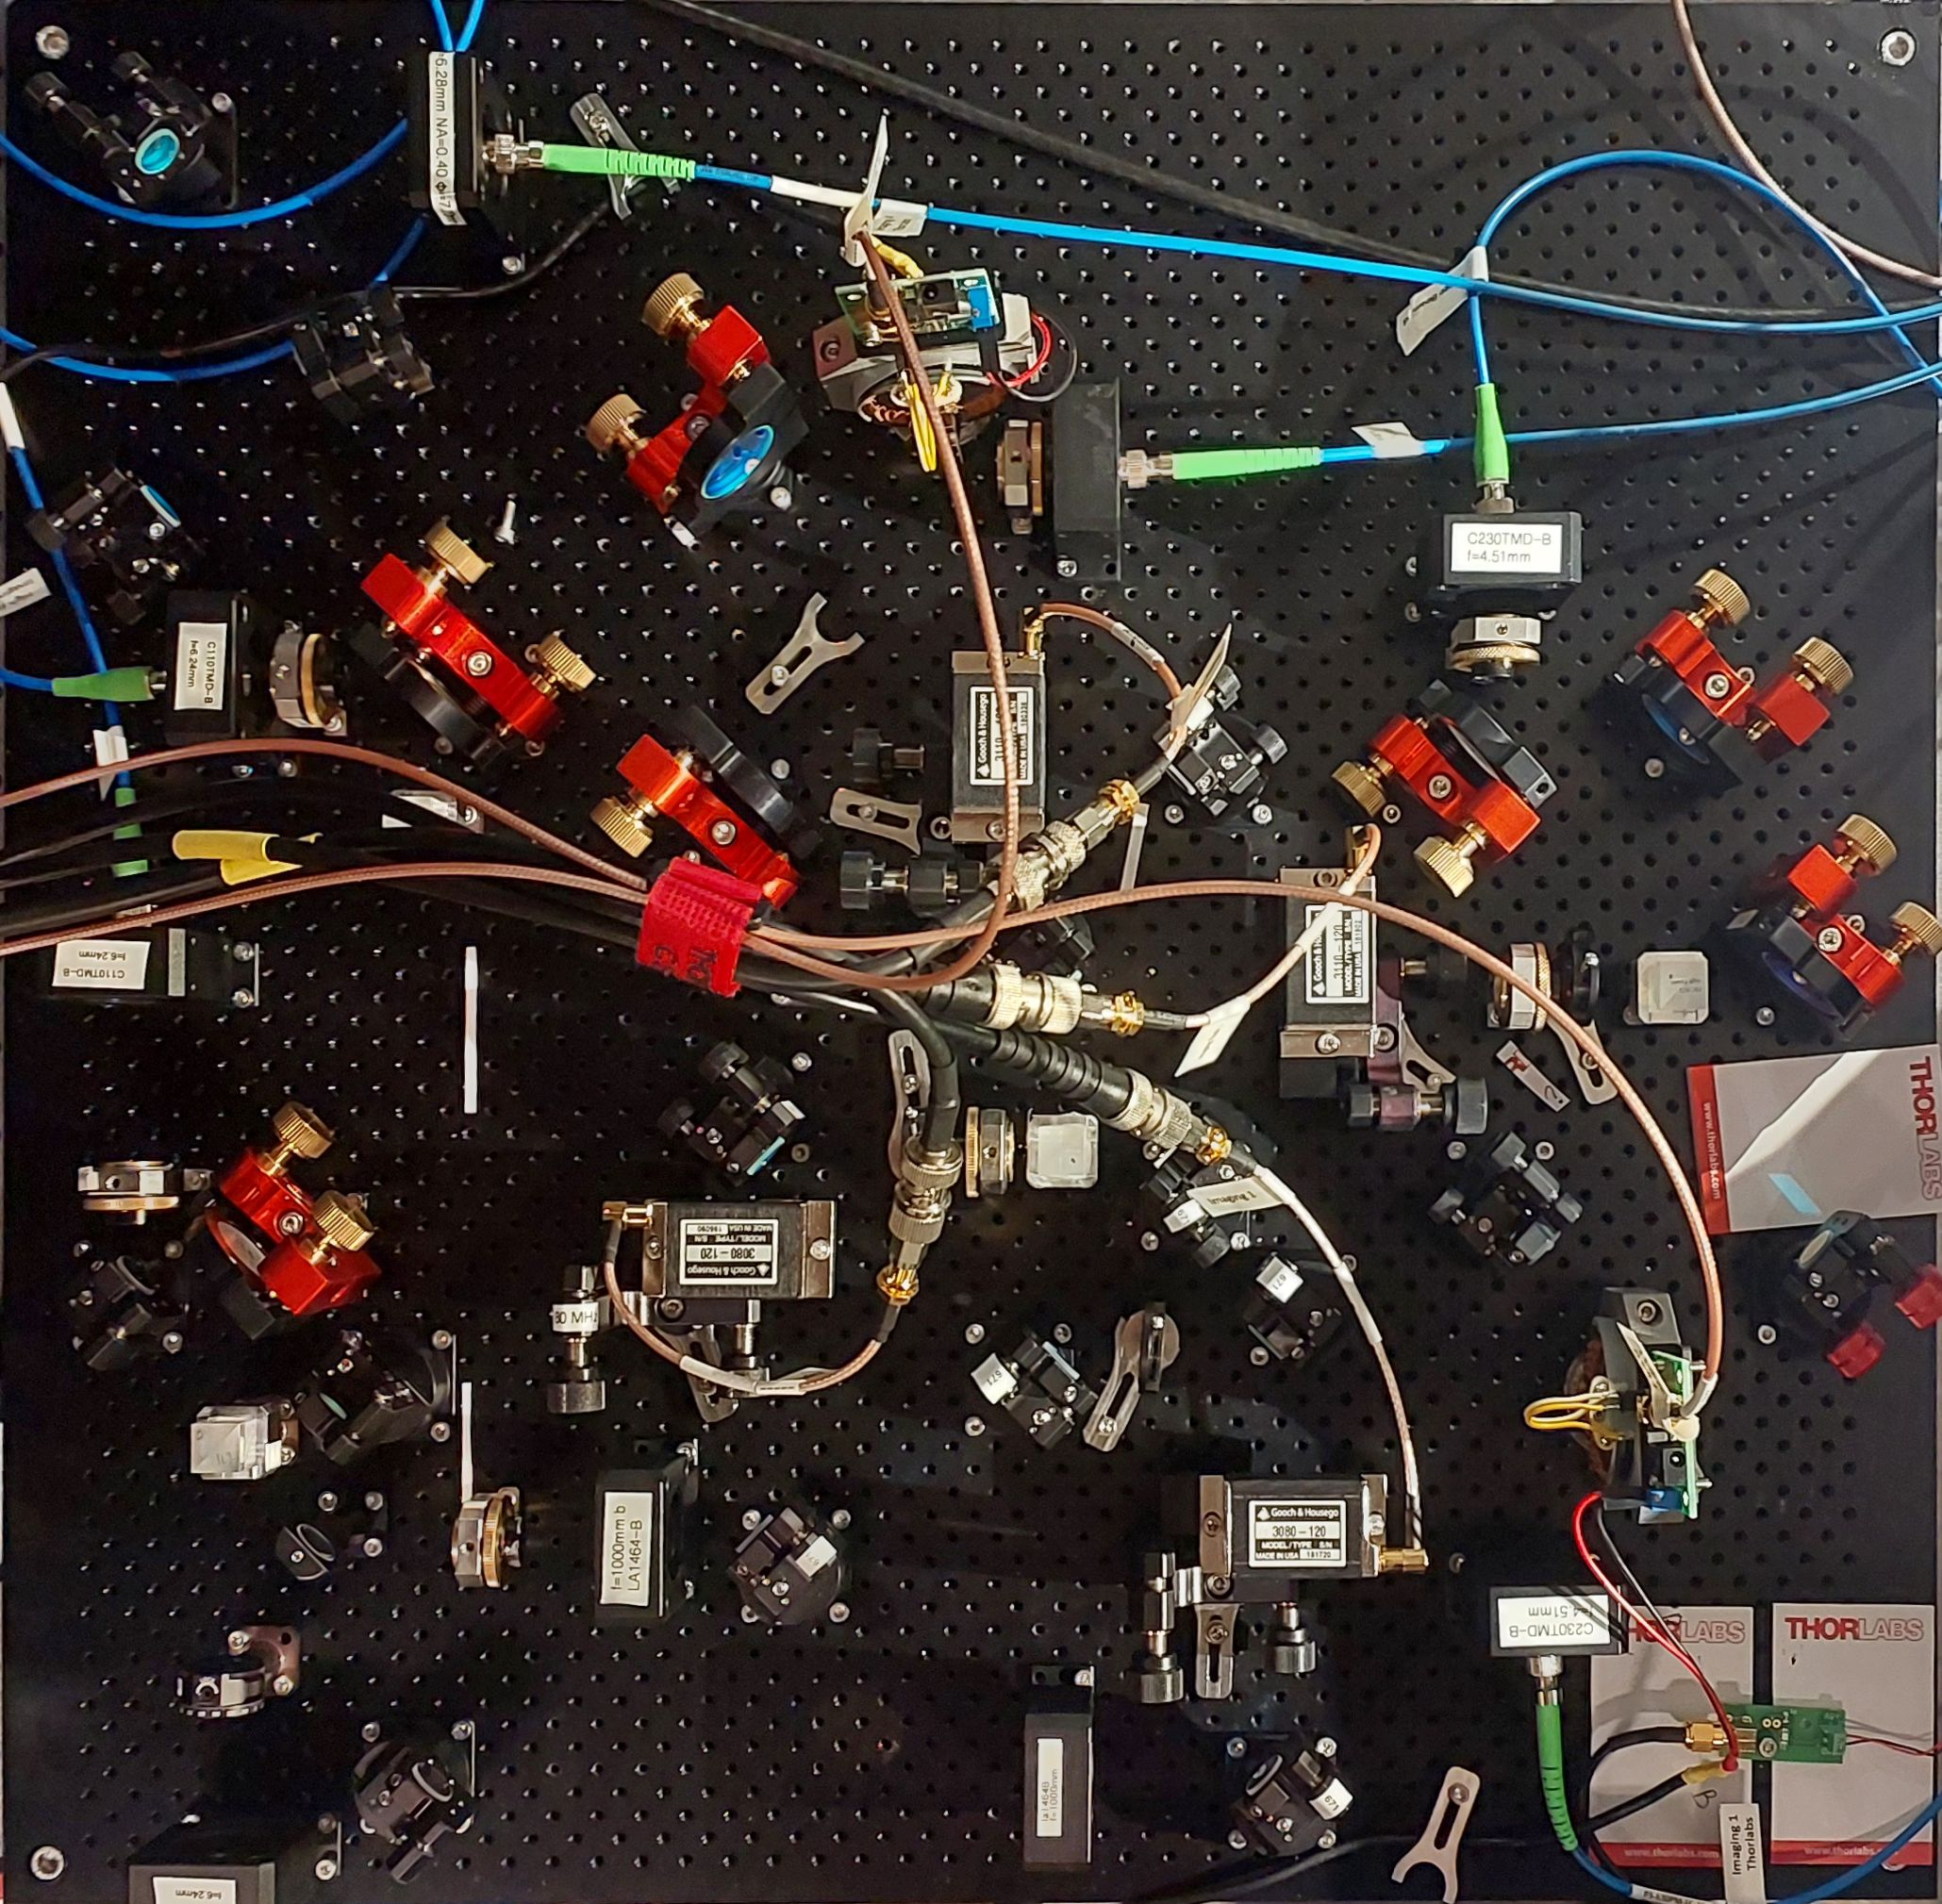
\includegraphics[width=0.4\textwidth]{imgs/flashing-distribution-img.jpg}

%     \addletter{90}{c}
%     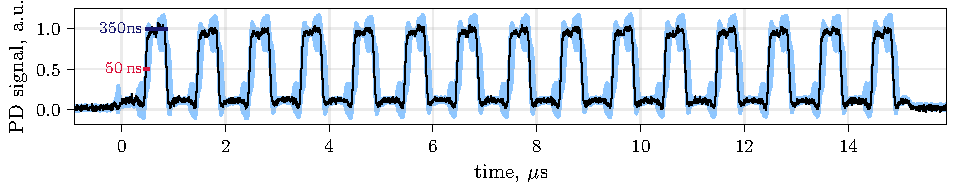
\includegraphics{fig-py/flashing-oscilloscope.pdf}

%     \caption{
%         \textbf{Distribution board for flashing}. 
%         a) Optical layout of the board used to combine and control light for free-space imaging states $\ket{3}$ and $\ket{6}$.
%         b) Experimental implementation.
%         c) PD signal of the flashing measured on an oscilloscope (black -- a single experimental run, blue -- the standard deviation over 20 runs, red -- rise time).
%     }
%     \label{fig:flashing}
% \end{figure}
